\section{Problem 2}

\subsection{Description Of The Attack}
The attacker is given $a = (a_1, ..., a_n)$, where $a_i = \sum_{j=1}^{i}a_j + Z_i$, and $Z_i$ are chosen uniformly at random from $\{0, 1\}$. \\

\noindent The attack is very simple: \begin{enumerate}
    \item Compute $z = \textit{leftPrefixSum}(a)$. \\
          Now $z = (a_1, a_1 + a_2, a_1 + a_2 + a_3, ...)$.
    \item Compute $z'$ such that $z'_i = z_i - i/2.0$ \\
          Because $z$ is a prefix sum, every entry $i$ contains the sum of all the random $Z_j$ for $j \leq i$.
          This is very helpful, although any single $Z_i$ can be either $0, 1$ with the same probability (and thus has relatively large variance), the sum of $k$ many such $Z_i$ has low variance, and expected value $k/2$. \\
          \textit{Intuition: With high probability, we have removed the noise from many entries (at least enough for rounding to be able to fix it)}
    \item Compute $b$ such that $b_i = z_i - z_{i-1}$ and $b_1 = z_1$. \\
          In effect, this undos step 1, making $b$ equal to the original prefix sums, with much of the noise removed. \\
    \item Let $A = ( A_{i,j} )$ such that $A_{i, j} = 1$ if $i \leq j$ and $0$ otherwise. \\
          This is a lower triangular matrix that contains only 1s in the lower part, and it match the prefix sum transformation.
    \item Efficiently Solve $A\hat{x} = b$ and perform rounding on elements of $\hat{x}$ to get the desired reconstruction.\\
          This step is very efficient because: (1) A is already in lower triangular form. (2) A has a special form where it contains 1 in all the lower part. A Forward pass can be executed in $O(n)$, by using a running accumulator/counter.
\end{enumerate}

\noindent I did not perform detailed analysis on the bounds of the error here, beyond the simple intuition about the variance of sums of many independent uniform binary variables, since I was able to test the accuracy empirically in the experiments. Given more time, I would be interested in carrying out such an analysis. \\

\noindent \textbf{Disclaimer:} I did not create another algorithm/attack for the case where additional information is known about $x$. I ran out of time, and the attack I have achieved the desired accuracy. I will try to come back to this soon to practice.

\begin{figure}
    \centering
    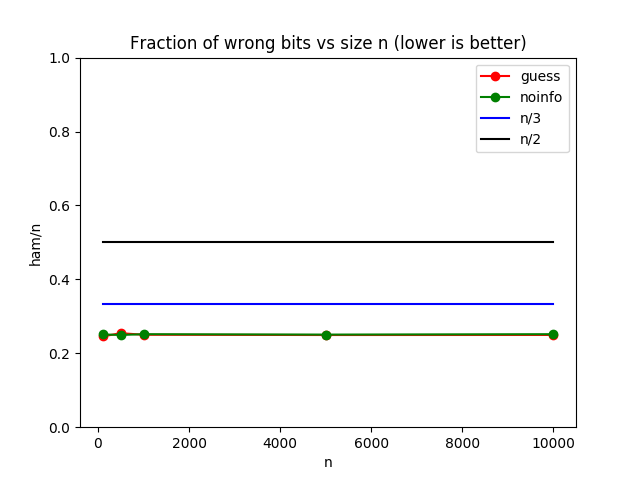
\includegraphics[width=\textwidth]{counter/all.png}
    \caption{Overall Accuracy for Problem 2 with and without additional info}
    \label{fig:counter}
\end{figure}

\subsection{Discussion}
In a sense, this is a form of composition, where several queries are being released about a data set as time progresses. The data set itself is ``logically'' changed, since new elements $x(i)$ are inserted into the sum with future queries (logically, this is as if such $x(i)$ was 0 in previous query). \\

\noindent It is very tricky to perform something like while preserving privacy without rigorous analysis. Especially to determine (1) the amount/distribution of noise, (2) the dependence/independence of noise between the several steps. \\

\noindent For example, even if the $Z_i$'s were not binary, but instead had some distribution over $\{1, ..., l \}$, the attack can still be carried through, by changing step (2) to remove the new expectation as opposed to $i/2$. This will probably result in some lower accuracy, but the attacker will still be able to reconstruct a decent portion of the data-set. \\

\noindent Instead, it seems like introducing some correlation or dependence between the different $Z_i$ can be a more interesting approach, as that will potentially increase the variance of the sum (e.g. cannot use independent to get the variance reduced to the sum of the individual variances). Utilizing this in addition to (moderatly) increasing the range of the $Z_i$'s could lead to significant improvement in privacy (the cost at utility is unclear to me right now).